\subsection{Imagen blocks}
\label{appendix:imagen}

\begin{figure}
    \centering
    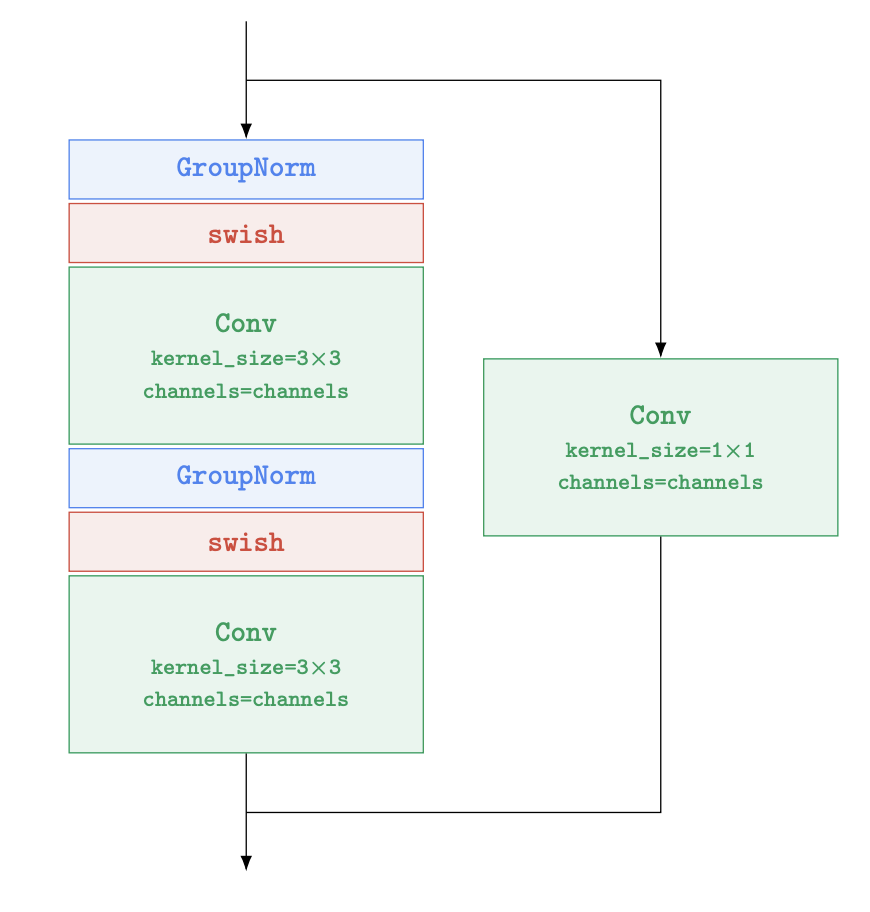
\includegraphics[width=0.5\textwidth]{images/appendix/imagen/unet_resnetblock.png}
    \caption{Imagen efficient U-Net \texttt{ResNetBlock} architecture.}
    \label{fig:appendix_imagen_resnetblock}
\end{figure}

In figure \ref{fig:appendix_imagen_resnetblock} we can see the \texttt{ResNetBlock} in use by Imagen (section \ref{sec:imagen}), by both the \texttt{DBlock} (downsampler) and the \texttt{UBlock} (the upsampler). The only input / hyperparameters of the \texttt{ResNetBlock} is the number of channels. The activation function is Swish (equation \ref{eq:appendix_activations_swish}).

\begin{figure*}
    \centering
    \begin{subfigure}[b]{0.5\textwidth}   
        \centering 
        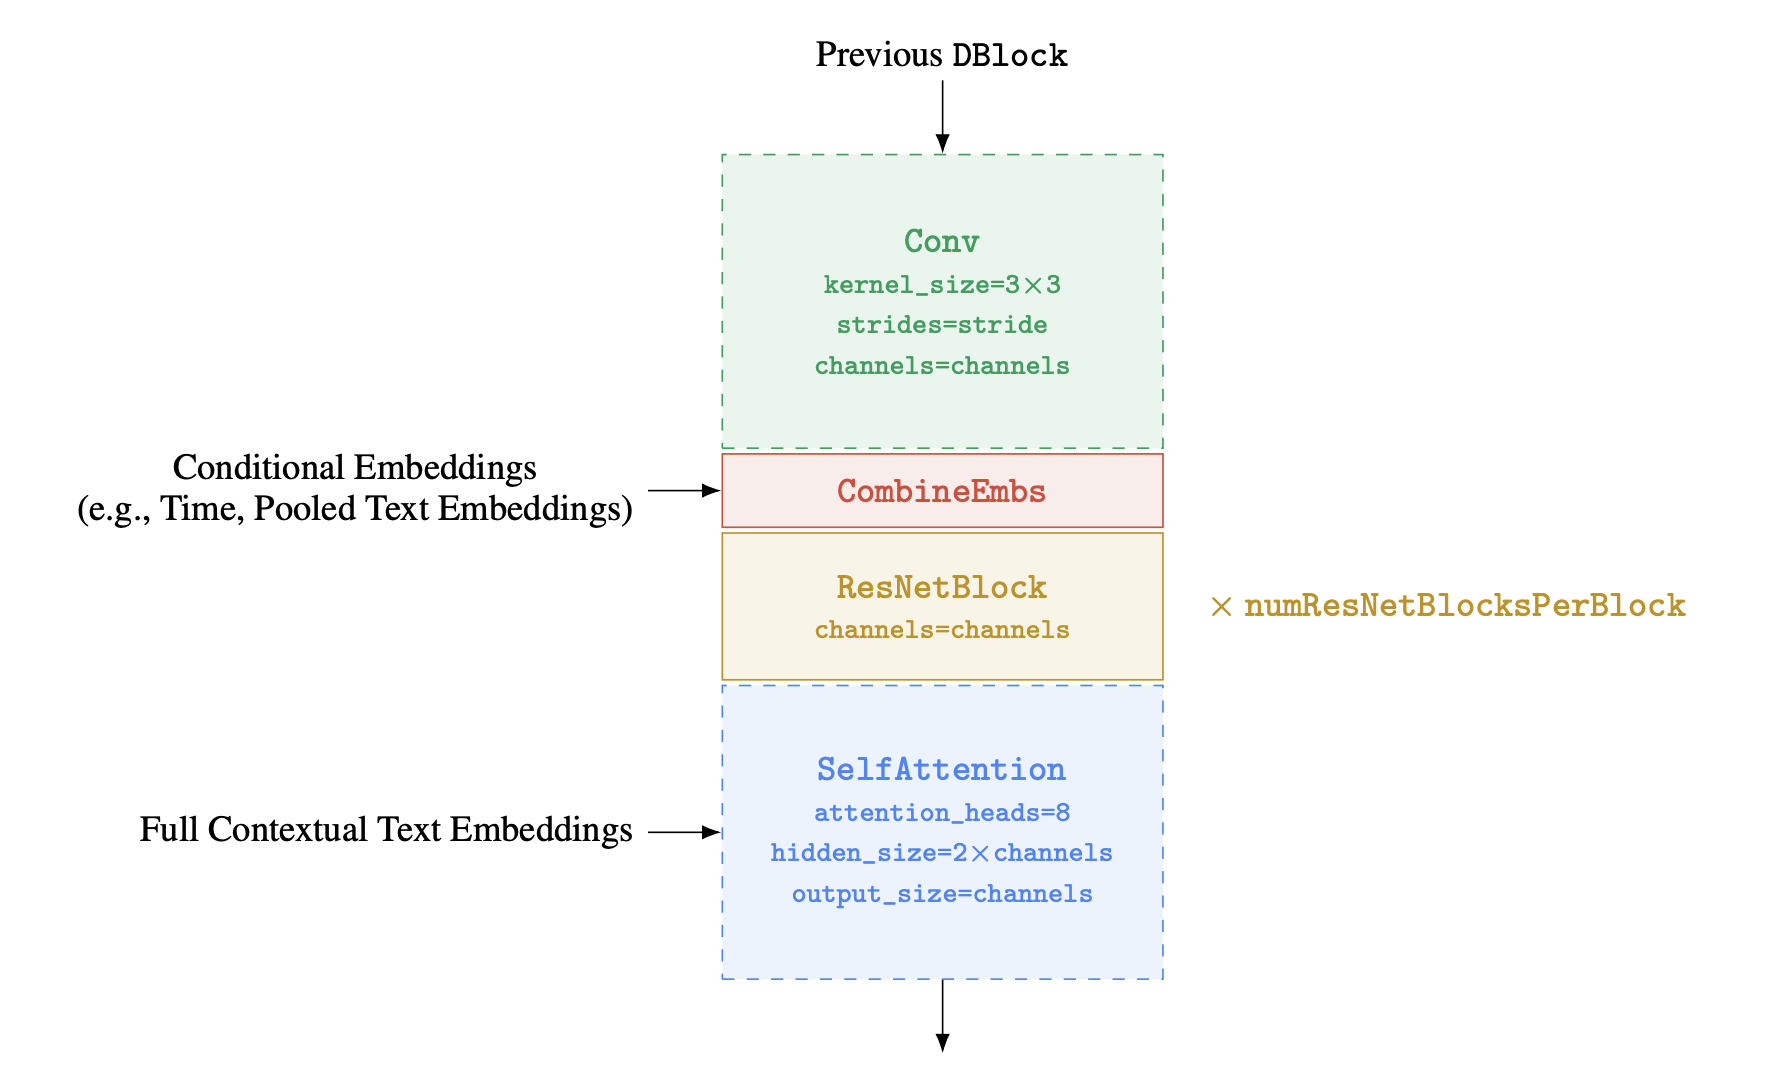
\includegraphics[width=\textwidth]{images/appendix/imagen/dblock.png}
        \caption[]%
        {{\small Imagen efficient U-Net \texttt{DBlock} architecture.}}
    \end{subfigure}
    \hfill
    \begin{subfigure}[b]{0.475\textwidth}
        \centering
        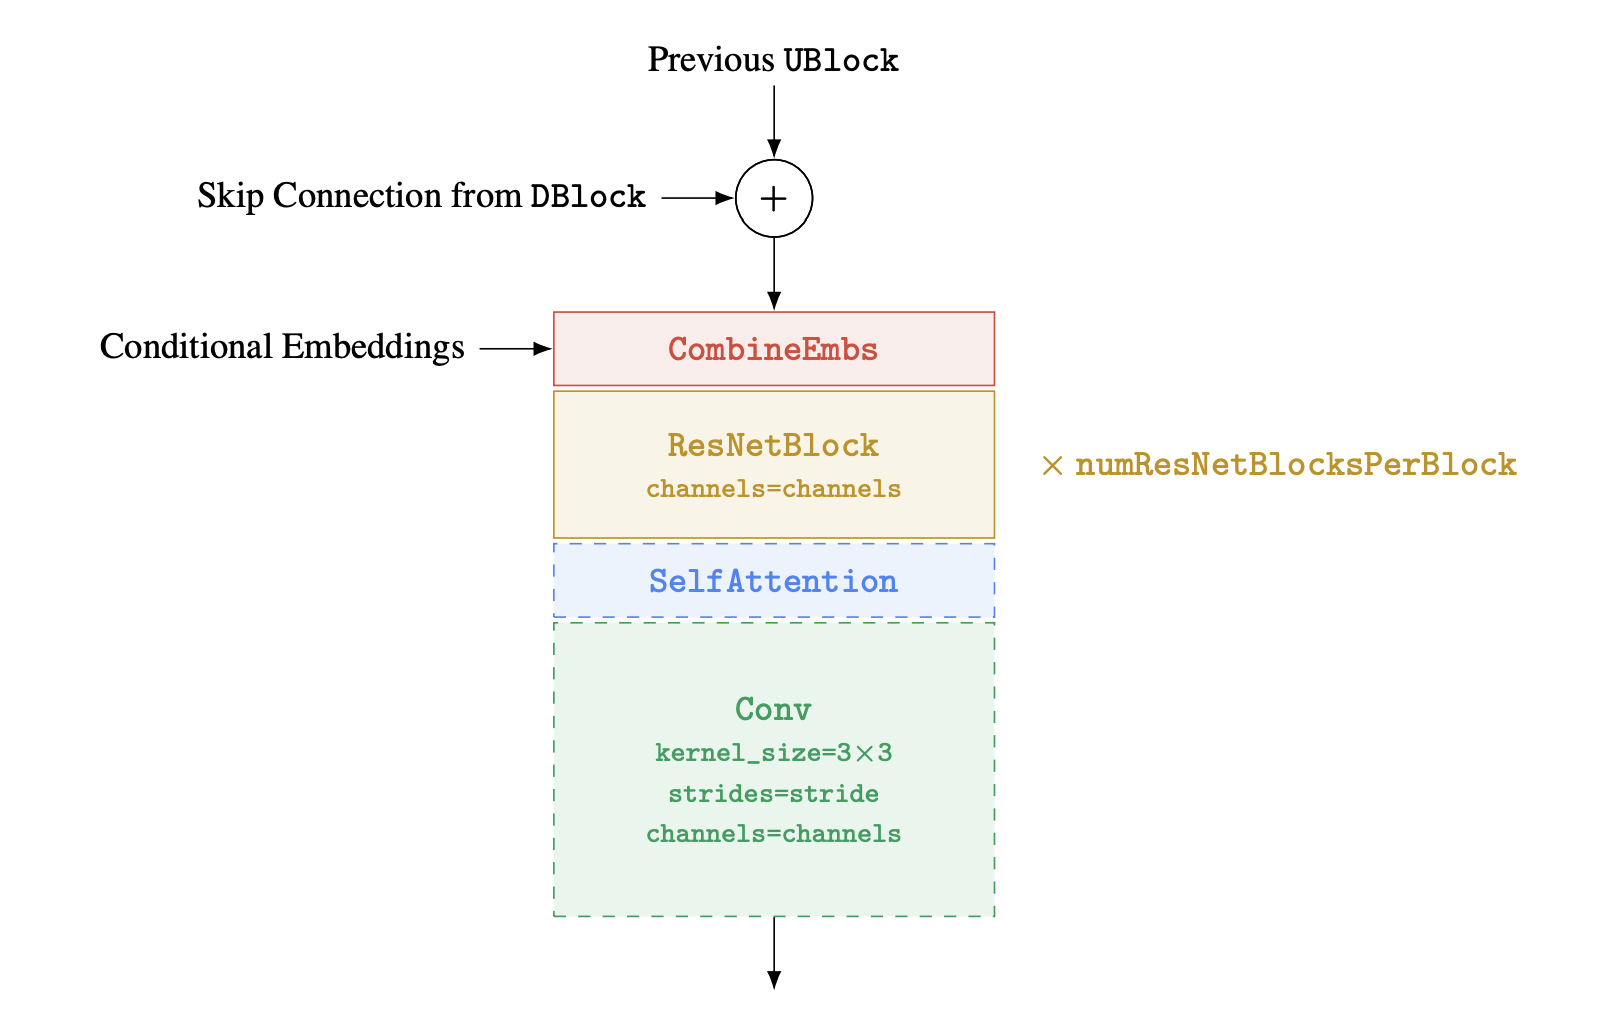
\includegraphics[width=\textwidth]{images/appendix/imagen/ublock.png}
        \caption[]%
        {{\small Imagen efficient U-Net \texttt{UBlock} architecture.}}
    \end{subfigure}
\end{figure*}


